\documentclass[1p]{elsarticle_modified}
%\bibliographystyle{elsarticle-num}

%\usepackage[colorlinks]{hyperref}
%\usepackage{abbrmath_seonhwa} %\Abb, \Ascr, \Acal ,\Abf, \Afrak
\usepackage{amsfonts}
\usepackage{amssymb}
\usepackage{amsmath}
\usepackage{amsthm}
\usepackage{scalefnt}
\usepackage{amsbsy}
\usepackage{kotex}
\usepackage{caption}
\usepackage{subfig}
\usepackage{color}
\usepackage{graphicx}
\usepackage{xcolor} %% white, black, red, green, blue, cyan, magenta, yellow
\usepackage{float}
\usepackage{setspace}
\usepackage{hyperref}

\usepackage{tikz}
\usetikzlibrary{arrows}

\usepackage{multirow}
\usepackage{array} % fixed length table
\usepackage{hhline}

%%%%%%%%%%%%%%%%%%%%%
\makeatletter
\renewcommand*\env@matrix[1][\arraystretch]{%
	\edef\arraystretch{#1}%
	\hskip -\arraycolsep
	\let\@ifnextchar\new@ifnextchar
	\array{*\c@MaxMatrixCols c}}
\makeatother %https://tex.stackexchange.com/questions/14071/how-can-i-increase-the-line-spacing-in-a-matrix
%%%%%%%%%%%%%%%

\usepackage[normalem]{ulem}

\newcommand{\msout}[1]{\ifmmode\text{\sout{\ensuremath{#1}}}\else\sout{#1}\fi}
%SOURCE: \msout is \stkout macro in https://tex.stackexchange.com/questions/20609/strikeout-in-math-mode

\newcommand{\cancel}[1]{
	\ifmmode
	{\color{red}\msout{#1}}
	\else
	{\color{red}\sout{#1}}
	\fi
}

\newcommand{\add}[1]{
	{\color{blue}\uwave{#1}}
}

\newcommand{\replace}[2]{
	\ifmmode
	{\color{red}\msout{#1}}{\color{blue}\uwave{#2}}
	\else
	{\color{red}\sout{#1}}{\color{blue}\uwave{#2}}
	\fi
}

\newcommand{\Sol}{\mathcal{S}} %segment
\newcommand{\D}{D} %diagram
\newcommand{\A}{\mathcal{A}} %arc


%%%%%%%%%%%%%%%%%%%%%%%%%%%%%5 test

\def\sl{\operatorname{\textup{SL}}(2,\Cbb)}
\def\psl{\operatorname{\textup{PSL}}(2,\Cbb)}
\def\quan{\mkern 1mu \triangleright \mkern 1mu}

\theoremstyle{definition}
\newtheorem{thm}{Theorem}[section]
\newtheorem{prop}[thm]{Proposition}
\newtheorem{lem}[thm]{Lemma}
\newtheorem{ques}[thm]{Question}
\newtheorem{cor}[thm]{Corollary}
\newtheorem{defn}[thm]{Definition}
\newtheorem{exam}[thm]{Example}
\newtheorem{rmk}[thm]{Remark}
\newtheorem{alg}[thm]{Algorithm}

\newcommand{\I}{\sqrt{-1}}
\begin{document}

%\begin{frontmatter}
%
%\title{Boundary parabolic representations of knots up to 8 crossings}
%
%%% Group authors per affiliation:
%\author{Yunhi Cho} 
%\address{Department of Mathematics, University of Seoul, Seoul, Korea}
%\ead{yhcho@uos.ac.kr}
%
%
%\author{Seonhwa Kim} %\fnref{s_kim}}
%\address{Center for Geometry and Physics, Institute for Basic Science, Pohang, 37673, Korea}
%\ead{ryeona17@ibs.re.kr}
%
%\author{Hyuk Kim}
%\address{Department of Mathematical Sciences, Seoul National University, Seoul 08826, Korea}
%\ead{hyukkim@snu.ac.kr}
%
%\author{Seokbeom Yoon}
%\address{Department of Mathematical Sciences, Seoul National University, Seoul, 08826,  Korea}
%\ead{sbyoon15@snu.ac.kr}
%
%\begin{abstract}
%We find all boundary parabolic representation of knots up to 8 crossings.
%
%\end{abstract}
%\begin{keyword}
%    \MSC[2010] 57M25 
%\end{keyword}
%
%\end{frontmatter}

%\linenumbers
%\tableofcontents
%
\newcommand\colored[1]{\textcolor{white}{\rule[-0.35ex]{0.8em}{1.4ex}}\kern-0.8em\color{red} #1}%
%\newcommand\colored[1]{\textcolor{white}{ #1}\kern-2.17ex	\textcolor{white}{ #1}\kern-1.81ex	\textcolor{white}{ #1}\kern-2.15ex\color{red}#1	}

{\Large $\underline{11a_{149}~(K11a_{149})}$}

\setlength{\tabcolsep}{10pt}
\renewcommand{\arraystretch}{1.6}
\vspace{1cm}\begin{tabular}{m{100pt}>{\centering\arraybackslash}m{274pt}}
\multirow{5}{120pt}{
	\centering
	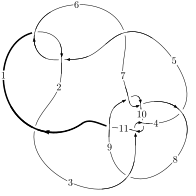
\includegraphics[width=112pt]{../../../GIT/diagram.site/Diagrams/png/398_11a_149.png}\\
\ \ \ A knot diagram\footnotemark}&
\allowdisplaybreaks
\textbf{Linearized knot diagam} \\
\cline{2-2}
 &
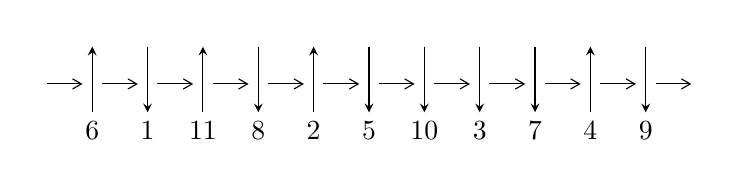
\begin{tikzpicture}[x=20pt, y=17pt]
	% nodes
	\node (C0) at (0, 0) {};
	\node (C1) at (1, 0) {};
	\node (C1U) at (1, +1) {};
	\node (C1D) at (1, -1) {6};

	\node (C2) at (2, 0) {};
	\node (C2U) at (2, +1) {};
	\node (C2D) at (2, -1) {1};

	\node (C3) at (3, 0) {};
	\node (C3U) at (3, +1) {};
	\node (C3D) at (3, -1) {11};

	\node (C4) at (4, 0) {};
	\node (C4U) at (4, +1) {};
	\node (C4D) at (4, -1) {8};

	\node (C5) at (5, 0) {};
	\node (C5U) at (5, +1) {};
	\node (C5D) at (5, -1) {2};

	\node (C6) at (6, 0) {};
	\node (C6U) at (6, +1) {};
	\node (C6D) at (6, -1) {5};

	\node (C7) at (7, 0) {};
	\node (C7U) at (7, +1) {};
	\node (C7D) at (7, -1) {10};

	\node (C8) at (8, 0) {};
	\node (C8U) at (8, +1) {};
	\node (C8D) at (8, -1) {3};

	\node (C9) at (9, 0) {};
	\node (C9U) at (9, +1) {};
	\node (C9D) at (9, -1) {7};

	\node (C10) at (10, 0) {};
	\node (C10U) at (10, +1) {};
	\node (C10D) at (10, -1) {4};

	\node (C11) at (11, 0) {};
	\node (C11U) at (11, +1) {};
	\node (C11D) at (11, -1) {9};
	\node (C12) at (12, 0) {};

	% arrows
	\draw[->,>={angle 60}]
	(C0) edge (C1) (C1) edge (C2) (C2) edge (C3) (C3) edge (C4) (C4) edge (C5) (C5) edge (C6) (C6) edge (C7) (C7) edge (C8) (C8) edge (C9) (C9) edge (C10) (C10) edge (C11) (C11) edge (C12) ;	\draw[->,>=stealth]
	(C1D) edge (C1U) (C2U) edge (C2D) (C3D) edge (C3U) (C4U) edge (C4D) (C5D) edge (C5U) (C6U) edge (C6D) (C7U) edge (C7D) (C8U) edge (C8D) (C9U) edge (C9D) (C10D) edge (C10U) (C11U) edge (C11D) ;
	\end{tikzpicture} \\
\hhline{~~} \\& 
\textbf{Solving Sequence} \\ \cline{2-2} 
 &
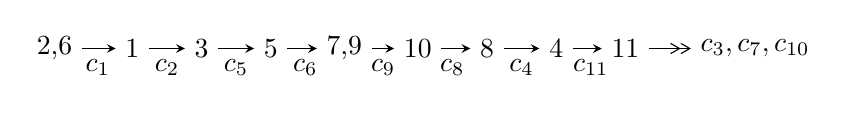
\begin{tikzpicture}[x=25pt, y=7pt]
	% node
	\node (A0) at (-1/8, 0) {2,6};
	\node (A1) at (1, 0) {1};
	\node (A2) at (2, 0) {3};
	\node (A3) at (3, 0) {5};
	\node (A4) at (65/16, 0) {7,9};
	\node (A5) at (41/8, 0) {10};
	\node (A6) at (49/8, 0) {8};
	\node (A7) at (57/8, 0) {4};
	\node (A8) at (65/8, 0) {11};
	\node (C1) at (1/2, -1) {$c_{1}$};
	\node (C2) at (3/2, -1) {$c_{2}$};
	\node (C3) at (5/2, -1) {$c_{5}$};
	\node (C4) at (7/2, -1) {$c_{6}$};
	\node (C5) at (37/8, -1) {$c_{9}$};
	\node (C6) at (45/8, -1) {$c_{8}$};
	\node (C7) at (53/8, -1) {$c_{4}$};
	\node (C8) at (61/8, -1) {$c_{11}$};
	\node (A9) at (10, 0) {$c_{3},c_{7},c_{10}$};

	% edge
	\draw[->,>=stealth]	
	(A0) edge (A1) (A1) edge (A2) (A2) edge (A3) (A3) edge (A4) (A4) edge (A5) (A5) edge (A6) (A6) edge (A7) (A7) edge (A8) ;
	\draw[->>,>={angle 60}]	
	(A8) edge (A9);
\end{tikzpicture} \\ 

\end{tabular} \\

\footnotetext{
The image of knot diagram is generated by the software ``\textbf{Draw programme}" developed by Andrew Bartholomew(\url{http://www.layer8.co.uk/maths/draw/index.htm\#Running-draw}), where we modified some parts for our purpose(\url{https://github.com/CATsTAILs/LinksPainter}).
}\phantom \\ \newline 
\centering \textbf{Ideals for irreducible components\footnotemark of $X_{\text{par}}$} 
 
\begin{align*}
I^u_{1}&=\langle 
6.59200\times10^{33} u^{62}+1.26617\times10^{34} u^{61}+\cdots+9.14845\times10^{33} b-6.13231\times10^{33},\\
\phantom{I^u_{1}}&\phantom{= \langle  }-5.18869\times10^{30} u^{62}-4.60084\times10^{31} u^{61}+\cdots+1.51632\times10^{32} a+4.89769\times10^{32},\;u^{63}+3 u^{62}+\cdots+2 u-1\rangle \\
\\
\end{align*}
\raggedright * 1 irreducible components of $\dim_{\mathbb{C}}=0$, with total 63 representations.\\
\footnotetext{All coefficients of polynomials are rational numbers. But the coefficients are sometimes approximated in decimal forms when there is not enough margin.}
\newpage
\renewcommand{\arraystretch}{1}
\centering \section*{I. $I^u_{1}= \langle 6.59\times10^{33} u^{62}+1.27\times10^{34} u^{61}+\cdots+9.15\times10^{33} b-6.13\times10^{33},\;-5.19\times10^{30} u^{62}-4.60\times10^{31} u^{61}+\cdots+1.52\times10^{32} a+4.90\times10^{32},\;u^{63}+3 u^{62}+\cdots+2 u-1 \rangle$}
\flushleft \textbf{(i) Arc colorings}\\
\begin{tabular}{m{7pt} m{180pt} m{7pt} m{180pt} }
\flushright $a_{2}=$&$\begin{pmatrix}1\\0\end{pmatrix}$ \\
\flushright $a_{6}=$&$\begin{pmatrix}0\\u\end{pmatrix}$ \\
\flushright $a_{1}=$&$\begin{pmatrix}1\\u^2\end{pmatrix}$ \\
\flushright $a_{3}=$&$\begin{pmatrix}u^2+1\\u^4\end{pmatrix}$ \\
\flushright $a_{5}=$&$\begin{pmatrix}- u\\u\end{pmatrix}$ \\
\flushright $a_{7}=$&$\begin{pmatrix}- u^3\\u^3+u\end{pmatrix}$ \\
\flushright $a_{9}=$&$\begin{pmatrix}0.0342190 u^{62}+0.303422 u^{61}+\cdots-0.970526 u-3.22999\\-0.720560 u^{62}-1.38403 u^{61}+\cdots+0.258985 u+0.670312\end{pmatrix}$ \\
\flushright $a_{10}=$&$\begin{pmatrix}0.163991 u^{62}+0.735688 u^{61}+\cdots-0.518791 u-3.41101\\-0.940033 u^{62}-1.90438 u^{61}+\cdots-0.942790 u+0.713453\end{pmatrix}$ \\
\flushright $a_{8}=$&$\begin{pmatrix}0.167447 u^{62}+0.652868 u^{61}+\cdots+1.09284 u-3.15598\\-0.702143 u^{62}-1.31297 u^{61}+\cdots+0.508662 u+0.602596\end{pmatrix}$ \\
\flushright $a_{4}=$&$\begin{pmatrix}-1.53220 u^{62}-5.33133 u^{61}+\cdots-6.95145 u+3.31985\\0.408926 u^{62}+1.90611 u^{61}+\cdots-1.94941 u+0.452963\end{pmatrix}$ \\
\flushright $a_{11}=$&$\begin{pmatrix}-0.489880 u^{62}-1.42153 u^{61}+\cdots+3.35861 u+3.51142\\-0.552392 u^{62}-2.69530 u^{61}+\cdots+2.86212 u-1.33768\end{pmatrix}$\\ \flushright $a_{11}=$&$\begin{pmatrix}-0.489880 u^{62}-1.42153 u^{61}+\cdots+3.35861 u+3.51142\\-0.552392 u^{62}-2.69530 u^{61}+\cdots+2.86212 u-1.33768\end{pmatrix}$\\&\end{tabular}
\flushleft \textbf{(ii) Obstruction class $= -1$}\\~\\
\flushleft \textbf{(iii) Cusp Shapes $= -2.55683 u^{62}-9.47657 u^{61}+\cdots-10.7932 u-4.31798$}\\~\\
\newpage\renewcommand{\arraystretch}{1}
\flushleft \textbf{(iv) u-Polynomials at the component}\newline \\
\begin{tabular}{m{50pt}|m{274pt}}
Crossings & \hspace{64pt}u-Polynomials at each crossing \\
\hline $$\begin{aligned}c_{1},c_{5}\end{aligned}$$&$\begin{aligned}
&u^{63}-3 u^{62}+\cdots+2 u+1
\end{aligned}$\\
\hline $$\begin{aligned}c_{2},c_{6}\end{aligned}$$&$\begin{aligned}
&u^{63}+19 u^{62}+\cdots+16 u-1
\end{aligned}$\\
\hline $$\begin{aligned}c_{3},c_{10}\end{aligned}$$&$\begin{aligned}
&u^{63}+3 u^{62}+\cdots+4 u+1
\end{aligned}$\\
\hline $$\begin{aligned}c_{4}\end{aligned}$$&$\begin{aligned}
&u^{63}+11 u^{62}+\cdots+26 u+529
\end{aligned}$\\
\hline $$\begin{aligned}c_{7},c_{9}\end{aligned}$$&$\begin{aligned}
&u^{63}- u^{62}+\cdots-18 u+1
\end{aligned}$\\
\hline $$\begin{aligned}c_{8}\end{aligned}$$&$\begin{aligned}
&u^{63}+u^{62}+\cdots-10 u+1
\end{aligned}$\\
\hline $$\begin{aligned}c_{11}\end{aligned}$$&$\begin{aligned}
&u^{63}+23 u^{62}+\cdots-22 u+1
\end{aligned}$\\
\hline
\end{tabular}\\~\\
\newpage\renewcommand{\arraystretch}{1}
\flushleft \textbf{(v) Riley Polynomials at the component}\newline \\
\begin{tabular}{m{50pt}|m{274pt}}
Crossings & \hspace{64pt}Riley Polynomials at each crossing \\
\hline $$\begin{aligned}c_{1},c_{5}\end{aligned}$$&$\begin{aligned}
&y^{63}+19 y^{62}+\cdots+16 y-1
\end{aligned}$\\
\hline $$\begin{aligned}c_{2},c_{6}\end{aligned}$$&$\begin{aligned}
&y^{63}+51 y^{62}+\cdots+360 y-1
\end{aligned}$\\
\hline $$\begin{aligned}c_{3},c_{10}\end{aligned}$$&$\begin{aligned}
&y^{63}+47 y^{62}+\cdots+16 y-1
\end{aligned}$\\
\hline $$\begin{aligned}c_{4}\end{aligned}$$&$\begin{aligned}
&y^{63}+127 y^{62}+\cdots-1368376 y-279841
\end{aligned}$\\
\hline $$\begin{aligned}c_{7},c_{9}\end{aligned}$$&$\begin{aligned}
&y^{63}-41 y^{62}+\cdots-184 y-1
\end{aligned}$\\
\hline $$\begin{aligned}c_{8}\end{aligned}$$&$\begin{aligned}
&y^{63}+3 y^{62}+\cdots-48 y-1
\end{aligned}$\\
\hline $$\begin{aligned}c_{11}\end{aligned}$$&$\begin{aligned}
&y^{63}-177 y^{62}+\cdots-84 y-1
\end{aligned}$\\
\hline
\end{tabular}\\~\\
\newpage\flushleft \textbf{(vi) Complex Volumes and Cusp Shapes}
$$\begin{array}{c|c|c}  
\text{Solutions to }I^u_{1}& \I (\text{vol} + \sqrt{-1}CS) & \text{Cusp shape}\\
 \hline 
\begin{aligned}
u &= \phantom{-}0.202849 + 0.946044 I \\
a &= \phantom{-}1.94722 + 0.19778 I \\
b &= -0.928613 - 0.106351 I\end{aligned}
 & -3.81545 + 5.01176 I & -9.09327 - 7.69438 I \\ \hline\begin{aligned}
u &= \phantom{-}0.202849 - 0.946044 I \\
a &= \phantom{-}1.94722 - 0.19778 I \\
b &= -0.928613 + 0.106351 I\end{aligned}
 & -3.81545 - 5.01176 I & -9.09327 + 7.69438 I \\ \hline\begin{aligned}
u &= \phantom{-}0.695239 + 0.763843 I \\
a &= \phantom{-}0.75961 + 1.41295 I \\
b &= -1.63934 + 0.73836 I\end{aligned}
 & -2.73449 - 1.42844 I & -6.93697 + 2.22951 I \\ \hline\begin{aligned}
u &= \phantom{-}0.695239 - 0.763843 I \\
a &= \phantom{-}0.75961 - 1.41295 I \\
b &= -1.63934 - 0.73836 I\end{aligned}
 & -2.73449 + 1.42844 I & -6.93697 - 2.22951 I \\ \hline\begin{aligned}
u &= -0.058839 + 0.948485 I \\
a &= -1.17043 + 1.85637 I \\
b &= \phantom{-}0.45196 - 1.56324 I\end{aligned}
 & -7.69919 - 2.07381 I & -15.2166 + 3.4603 I \\ \hline\begin{aligned}
u &= -0.058839 - 0.948485 I \\
a &= -1.17043 - 1.85637 I \\
b &= \phantom{-}0.45196 + 1.56324 I\end{aligned}
 & -7.69919 + 2.07381 I & -15.2166 - 3.4603 I \\ \hline\begin{aligned}
u &= -0.763248 + 0.536252 I \\
a &= -0.200295 - 0.850847 I \\
b &= -0.612392 + 0.572188 I\end{aligned}
 & \phantom{-}1.08095 - 1.39801 I & \phantom{-}4.18188 + 0.71132 I \\ \hline\begin{aligned}
u &= -0.763248 - 0.536252 I \\
a &= -0.200295 + 0.850847 I \\
b &= -0.612392 - 0.572188 I\end{aligned}
 & \phantom{-}1.08095 + 1.39801 I & \phantom{-}4.18188 - 0.71132 I \\ \hline\begin{aligned}
u &= -0.726705 + 0.811867 I \\
a &= -1.18396 + 1.72005 I \\
b &= \phantom{-}2.18880 + 0.14253 I\end{aligned}
 & \phantom{-}1.35473 - 0.62400 I & \phantom{-0.000000 } 0 \\ \hline\begin{aligned}
u &= -0.726705 - 0.811867 I \\
a &= -1.18396 - 1.72005 I \\
b &= \phantom{-}2.18880 - 0.14253 I\end{aligned}
 & \phantom{-}1.35473 + 0.62400 I & \phantom{-0.000000 } 0\\
 \hline 
 \end{array}$$\newpage$$\begin{array}{c|c|c}  
\text{Solutions to }I^u_{1}& \I (\text{vol} + \sqrt{-1}CS) & \text{Cusp shape}\\
 \hline 
\begin{aligned}
u &= -0.643524 + 0.884288 I \\
a &= -0.670137 + 0.681552 I \\
b &= -0.214774 + 0.538469 I\end{aligned}
 & -4.63310 - 2.49365 I & \phantom{-0.000000 } 0 \\ \hline\begin{aligned}
u &= -0.643524 - 0.884288 I \\
a &= -0.670137 - 0.681552 I \\
b &= -0.214774 - 0.538469 I\end{aligned}
 & -4.63310 + 2.49365 I & \phantom{-0.000000 } 0 \\ \hline\begin{aligned}
u &= -0.810251 + 0.764677 I \\
a &= -0.614704 + 1.099300 I \\
b &= \phantom{-}2.27585 - 0.14042 I\end{aligned}
 & \phantom{-}2.66441 + 3.76429 I & \phantom{-0.000000 } 0 \\ \hline\begin{aligned}
u &= -0.810251 - 0.764677 I \\
a &= -0.614704 - 1.099300 I \\
b &= \phantom{-}2.27585 + 0.14042 I\end{aligned}
 & \phantom{-}2.66441 - 3.76429 I & \phantom{-0.000000 } 0 \\ \hline\begin{aligned}
u &= -0.247037 + 0.849494 I \\
a &= -1.142120 + 0.110784 I \\
b &= \phantom{-}0.398886 + 0.218053 I\end{aligned}
 & -0.62170 - 1.75556 I & -1.86458 + 4.77709 I \\ \hline\begin{aligned}
u &= -0.247037 - 0.849494 I \\
a &= -1.142120 - 0.110784 I \\
b &= \phantom{-}0.398886 - 0.218053 I\end{aligned}
 & -0.62170 + 1.75556 I & -1.86458 - 4.77709 I \\ \hline\begin{aligned}
u &= \phantom{-}0.879352 + 0.689382 I \\
a &= -0.766895 - 1.133880 I \\
b &= \phantom{-}1.80952 - 0.12559 I\end{aligned}
 & \phantom{-}3.67279 - 4.73223 I & \phantom{-0.000000 } 0 \\ \hline\begin{aligned}
u &= \phantom{-}0.879352 - 0.689382 I \\
a &= -0.766895 + 1.133880 I \\
b &= \phantom{-}1.80952 + 0.12559 I\end{aligned}
 & \phantom{-}3.67279 + 4.73223 I & \phantom{-0.000000 } 0 \\ \hline\begin{aligned}
u &= \phantom{-}0.702468 + 0.874127 I \\
a &= -1.37569 + 1.38479 I \\
b &= \phantom{-}0.83063 - 1.81611 I\end{aligned}
 & -0.03120 + 2.69612 I & \phantom{-0.000000 } 0 \\ \hline\begin{aligned}
u &= \phantom{-}0.702468 - 0.874127 I \\
a &= -1.37569 - 1.38479 I \\
b &= \phantom{-}0.83063 + 1.81611 I\end{aligned}
 & -0.03120 - 2.69612 I & \phantom{-0.000000 } 0\\
 \hline 
 \end{array}$$\newpage$$\begin{array}{c|c|c}  
\text{Solutions to }I^u_{1}& \I (\text{vol} + \sqrt{-1}CS) & \text{Cusp shape}\\
 \hline 
\begin{aligned}
u &= \phantom{-}0.057802 + 0.865842 I \\
a &= \phantom{-}1.039560 + 0.717759 I \\
b &= \phantom{-}0.212381 - 1.286120 I\end{aligned}
 & -3.45347 + 0.91963 I & -7.53722 + 0.57993 I \\ \hline\begin{aligned}
u &= \phantom{-}0.057802 - 0.865842 I \\
a &= \phantom{-}1.039560 - 0.717759 I \\
b &= \phantom{-}0.212381 + 1.286120 I\end{aligned}
 & -3.45347 - 0.91963 I & -7.53722 - 0.57993 I \\ \hline\begin{aligned}
u &= -0.888598 + 0.712739 I \\
a &= \phantom{-}1.23888 - 1.07985 I \\
b &= -2.21959 - 0.66956 I\end{aligned}
 & -1.25936 + 10.13510 I & \phantom{-0.000000 } 0 \\ \hline\begin{aligned}
u &= -0.888598 - 0.712739 I \\
a &= \phantom{-}1.23888 + 1.07985 I \\
b &= -2.21959 + 0.66956 I\end{aligned}
 & -1.25936 - 10.13510 I & \phantom{-0.000000 } 0 \\ \hline\begin{aligned}
u &= \phantom{-}0.737082 + 0.871113 I \\
a &= -4.8258 + 13.5054 I \\
b &= -5.4391 - 15.0888 I\end{aligned}
 & -0.27910 + 2.80205 I & \phantom{-0.000000 } 0. - 114.9176 I \\ \hline\begin{aligned}
u &= \phantom{-}0.737082 - 0.871113 I \\
a &= -4.8258 - 13.5054 I \\
b &= -5.4391 + 15.0888 I\end{aligned}
 & -0.27910 - 2.80205 I & \phantom{-0.000000 -}0. + 114.9176 I \\ \hline\begin{aligned}
u &= \phantom{-}0.249599 + 1.117340 I \\
a &= -0.933405 - 0.391979 I \\
b &= \phantom{-}0.083836 + 0.726791 I\end{aligned}
 & -8.93201 + 10.19930 I & \phantom{-0.000000 } 0 \\ \hline\begin{aligned}
u &= \phantom{-}0.249599 - 1.117340 I \\
a &= -0.933405 + 0.391979 I \\
b &= \phantom{-}0.083836 - 0.726791 I\end{aligned}
 & -8.93201 - 10.19930 I & \phantom{-0.000000 } 0 \\ \hline\begin{aligned}
u &= \phantom{-}0.825588 + 0.794026 I \\
a &= \phantom{-}0.471370 + 0.782650 I \\
b &= -1.65611 - 0.24031 I\end{aligned}
 & \phantom{-}6.05392 + 0.28945 I & \phantom{-0.000000 } 0 \\ \hline\begin{aligned}
u &= \phantom{-}0.825588 - 0.794026 I \\
a &= \phantom{-}0.471370 - 0.782650 I \\
b &= -1.65611 + 0.24031 I\end{aligned}
 & \phantom{-}6.05392 - 0.28945 I & \phantom{-0.000000 } 0\\
 \hline 
 \end{array}$$\newpage$$\begin{array}{c|c|c}  
\text{Solutions to }I^u_{1}& \I (\text{vol} + \sqrt{-1}CS) & \text{Cusp shape}\\
 \hline 
\begin{aligned}
u &= \phantom{-}0.171535 + 0.833363 I \\
a &= \phantom{-}0.472085 + 1.258500 I \\
b &= \phantom{-}0.192482 + 0.304858 I\end{aligned}
 & -3.56857 - 0.47654 I & -9.76423 - 1.75847 I \\ \hline\begin{aligned}
u &= \phantom{-}0.171535 - 0.833363 I \\
a &= \phantom{-}0.472085 - 1.258500 I \\
b &= \phantom{-}0.192482 - 0.304858 I\end{aligned}
 & -3.56857 + 0.47654 I & -9.76423 + 1.75847 I \\ \hline\begin{aligned}
u &= -0.716350 + 0.922760 I \\
a &= \phantom{-}0.58105 - 1.92526 I \\
b &= -2.53241 + 1.12922 I\end{aligned}
 & \phantom{-}1.01466 - 4.89030 I & \phantom{-0.000000 } 0 \\ \hline\begin{aligned}
u &= -0.716350 - 0.922760 I \\
a &= \phantom{-}0.58105 + 1.92526 I \\
b &= -2.53241 - 1.12922 I\end{aligned}
 & \phantom{-}1.01466 + 4.89030 I & \phantom{-0.000000 } 0 \\ \hline\begin{aligned}
u &= \phantom{-}0.693599 + 0.946330 I \\
a &= \phantom{-}0.34808 - 1.75912 I \\
b &= \phantom{-}1.94341 + 1.34022 I\end{aligned}
 & -3.28750 + 6.79142 I & \phantom{-0.000000 } 0 \\ \hline\begin{aligned}
u &= \phantom{-}0.693599 - 0.946330 I \\
a &= \phantom{-}0.34808 + 1.75912 I \\
b &= \phantom{-}1.94341 - 1.34022 I\end{aligned}
 & -3.28750 - 6.79142 I & \phantom{-0.000000 } 0 \\ \hline\begin{aligned}
u &= -0.765357 + 0.893742 I \\
a &= -0.888237 - 0.881040 I \\
b &= \phantom{-}0.160327 + 1.374950 I\end{aligned}
 & \phantom{-}1.42211 - 2.89988 I & \phantom{-0.000000 } 0 \\ \hline\begin{aligned}
u &= -0.765357 - 0.893742 I \\
a &= -0.888237 + 0.881040 I \\
b &= \phantom{-}0.160327 - 1.374950 I\end{aligned}
 & \phantom{-}1.42211 + 2.89988 I & \phantom{-0.000000 } 0 \\ \hline\begin{aligned}
u &= \phantom{-}0.818503 + 0.071595 I \\
a &= \phantom{-}0.947693 - 0.595880 I \\
b &= -0.190373 + 0.433337 I\end{aligned}
 & -4.90960 + 6.71055 I & -4.57662 - 5.93806 I \\ \hline\begin{aligned}
u &= \phantom{-}0.818503 - 0.071595 I \\
a &= \phantom{-}0.947693 + 0.595880 I \\
b &= -0.190373 - 0.433337 I\end{aligned}
 & -4.90960 - 6.71055 I & -4.57662 + 5.93806 I\\
 \hline 
 \end{array}$$\newpage$$\begin{array}{c|c|c}  
\text{Solutions to }I^u_{1}& \I (\text{vol} + \sqrt{-1}CS) & \text{Cusp shape}\\
 \hline 
\begin{aligned}
u &= \phantom{-}0.330834 + 1.132940 I \\
a &= \phantom{-}0.122863 - 0.871157 I \\
b &= -0.389791 + 0.792565 I\end{aligned}
 & -8.44469 - 2.66782 I & \phantom{-0.000000 } 0 \\ \hline\begin{aligned}
u &= \phantom{-}0.330834 - 1.132940 I \\
a &= \phantom{-}0.122863 + 0.871157 I \\
b &= -0.389791 - 0.792565 I\end{aligned}
 & -8.44469 + 2.66782 I & \phantom{-0.000000 } 0 \\ \hline\begin{aligned}
u &= -0.213920 + 1.163890 I \\
a &= \phantom{-}0.446939 - 0.170107 I \\
b &= \phantom{-}0.032442 + 0.590549 I\end{aligned}
 & -3.79459 - 4.37631 I & \phantom{-0.000000 } 0 \\ \hline\begin{aligned}
u &= -0.213920 - 1.163890 I \\
a &= \phantom{-}0.446939 + 0.170107 I \\
b &= \phantom{-}0.032442 - 0.590549 I\end{aligned}
 & -3.79459 + 4.37631 I & \phantom{-0.000000 } 0 \\ \hline\begin{aligned}
u &= -0.750069 + 0.975450 I \\
a &= \phantom{-}0.85338 - 2.02212 I \\
b &= -2.24959 + 0.46334 I\end{aligned}
 & \phantom{-}2.01737 - 9.62566 I & \phantom{-0.000000 } 0 \\ \hline\begin{aligned}
u &= -0.750069 - 0.975450 I \\
a &= \phantom{-}0.85338 + 2.02212 I \\
b &= -2.24959 - 0.46334 I\end{aligned}
 & \phantom{-}2.01737 + 9.62566 I & \phantom{-0.000000 } 0 \\ \hline\begin{aligned}
u &= \phantom{-}0.769036 + 0.963922 I \\
a &= -0.64711 - 1.44598 I \\
b &= \phantom{-}1.56684 + 0.33213 I\end{aligned}
 & \phantom{-}5.52656 + 5.67817 I & \phantom{-0.000000 } 0 \\ \hline\begin{aligned}
u &= \phantom{-}0.769036 - 0.963922 I \\
a &= -0.64711 + 1.44598 I \\
b &= \phantom{-}1.56684 - 0.33213 I\end{aligned}
 & \phantom{-}5.52656 - 5.67817 I & \phantom{-0.000000 } 0 \\ \hline\begin{aligned}
u &= -0.693016 + 0.315312 I \\
a &= -0.289428 - 0.730127 I \\
b &= -0.310255 + 0.482151 I\end{aligned}
 & \phantom{-}1.05806 - 1.32640 I & \phantom{-}4.87847 + 4.20428 I \\ \hline\begin{aligned}
u &= -0.693016 - 0.315312 I \\
a &= -0.289428 + 0.730127 I \\
b &= -0.310255 - 0.482151 I\end{aligned}
 & \phantom{-}1.05806 + 1.32640 I & \phantom{-}4.87847 - 4.20428 I\\
 \hline 
 \end{array}$$\newpage$$\begin{array}{c|c|c}  
\text{Solutions to }I^u_{1}& \I (\text{vol} + \sqrt{-1}CS) & \text{Cusp shape}\\
 \hline 
\begin{aligned}
u &= \phantom{-}0.754175 + 1.039690 I \\
a &= \phantom{-}0.72880 + 1.66445 I \\
b &= -2.16012 - 0.87201 I\end{aligned}
 & \phantom{-}2.59510 + 10.79480 I & \phantom{-0.000000 } 0 \\ \hline\begin{aligned}
u &= \phantom{-}0.754175 - 1.039690 I \\
a &= \phantom{-}0.72880 - 1.66445 I \\
b &= -2.16012 + 0.87201 I\end{aligned}
 & \phantom{-}2.59510 - 10.79480 I & \phantom{-0.000000 } 0 \\ \hline\begin{aligned}
u &= -0.765933 + 1.033730 I \\
a &= -0.51162 + 2.20505 I \\
b &= \phantom{-}2.40984 - 1.47160 I\end{aligned}
 & -2.2561 - 16.2663 I & \phantom{-0.000000 } 0 \\ \hline\begin{aligned}
u &= -0.765933 - 1.033730 I \\
a &= -0.51162 - 2.20505 I \\
b &= \phantom{-}2.40984 + 1.47160 I\end{aligned}
 & -2.2561 + 16.2663 I & \phantom{-0.000000 } 0 \\ \hline\begin{aligned}
u &= -0.933450 + 0.887239 I \\
a &= \phantom{-}0.182597 + 0.083461 I \\
b &= \phantom{-}0.164371 - 0.473416 I\end{aligned}
 & \phantom{-}0.88299 - 3.37440 I & \phantom{-0.000000 } 0 \\ \hline\begin{aligned}
u &= -0.933450 - 0.887239 I \\
a &= \phantom{-}0.182597 - 0.083461 I \\
b &= \phantom{-}0.164371 + 0.473416 I\end{aligned}
 & \phantom{-}0.88299 + 3.37440 I & \phantom{-0.000000 } 0 \\ \hline\begin{aligned}
u &= -0.730193 + 1.099430 I \\
a &= -0.467025 + 0.660302 I \\
b &= \phantom{-}1.157580 - 0.273573 I\end{aligned}
 & -0.60454 - 4.40493 I & \phantom{-0.000000 } 0 \\ \hline\begin{aligned}
u &= -0.730193 - 1.099430 I \\
a &= -0.467025 - 0.660302 I \\
b &= \phantom{-}1.157580 + 0.273573 I\end{aligned}
 & -0.60454 + 4.40493 I & \phantom{-0.000000 } 0 \\ \hline\begin{aligned}
u &= \phantom{-}0.516941 + 0.032452 I \\
a &= -0.286237 - 1.236950 I \\
b &= \phantom{-}0.641012 + 0.482457 I\end{aligned}
 & -1.03804 - 2.55802 I & -0.30006 + 3.39194 I \\ \hline\begin{aligned}
u &= \phantom{-}0.516941 - 0.032452 I \\
a &= -0.286237 + 1.236950 I \\
b &= \phantom{-}0.641012 - 0.482457 I\end{aligned}
 & -1.03804 + 2.55802 I & -0.30006 - 3.39194 I\\
 \hline 
 \end{array}$$\newpage$$\begin{array}{c|c|c}  
\text{Solutions to }I^u_{1}& \I (\text{vol} + \sqrt{-1}CS) & \text{Cusp shape}\\
 \hline 
\begin{aligned}
u &= -0.309755 + 0.275620 I \\
a &= \phantom{-}1.19826 + 2.47111 I \\
b &= -0.692520 + 0.579657 I\end{aligned}
 & -4.36178 - 1.13101 I & -3.69450 + 1.07714 I \\ \hline\begin{aligned}
u &= -0.309755 - 0.275620 I \\
a &= \phantom{-}1.19826 - 2.47111 I \\
b &= -0.692520 - 0.579657 I\end{aligned}
 & -4.36178 + 1.13101 I & -3.69450 - 1.07714 I \\ \hline\begin{aligned}
u &= \phantom{-}0.223288\phantom{ +0.000000I} \\
a &= -3.73067\phantom{ +0.000000I} \\
b &= \phantom{-}0.429527\phantom{ +0.000000I}\end{aligned}
 & -1.26040\phantom{ +0.000000I} & -8.85590\phantom{ +0.000000I}\\
 \hline 
 \end{array}$$\newpage
\newpage\renewcommand{\arraystretch}{1}
\centering \section*{ II. u-Polynomials}
\begin{tabular}{m{50pt}|m{274pt}}
Crossings & \hspace{64pt}u-Polynomials at each crossing \\
\hline $$\begin{aligned}c_{1},c_{5}\end{aligned}$$&$\begin{aligned}
&u^{63}-3 u^{62}+\cdots+2 u+1
\end{aligned}$\\
\hline $$\begin{aligned}c_{2},c_{6}\end{aligned}$$&$\begin{aligned}
&u^{63}+19 u^{62}+\cdots+16 u-1
\end{aligned}$\\
\hline $$\begin{aligned}c_{3},c_{10}\end{aligned}$$&$\begin{aligned}
&u^{63}+3 u^{62}+\cdots+4 u+1
\end{aligned}$\\
\hline $$\begin{aligned}c_{4}\end{aligned}$$&$\begin{aligned}
&u^{63}+11 u^{62}+\cdots+26 u+529
\end{aligned}$\\
\hline $$\begin{aligned}c_{7},c_{9}\end{aligned}$$&$\begin{aligned}
&u^{63}- u^{62}+\cdots-18 u+1
\end{aligned}$\\
\hline $$\begin{aligned}c_{8}\end{aligned}$$&$\begin{aligned}
&u^{63}+u^{62}+\cdots-10 u+1
\end{aligned}$\\
\hline $$\begin{aligned}c_{11}\end{aligned}$$&$\begin{aligned}
&u^{63}+23 u^{62}+\cdots-22 u+1
\end{aligned}$\\
\hline
\end{tabular}\newpage\renewcommand{\arraystretch}{1}
\centering \section*{ III. Riley Polynomials}
\begin{tabular}{m{50pt}|m{274pt}}
Crossings & \hspace{64pt}Riley Polynomials at each crossing \\
\hline $$\begin{aligned}c_{1},c_{5}\end{aligned}$$&$\begin{aligned}
&y^{63}+19 y^{62}+\cdots+16 y-1
\end{aligned}$\\
\hline $$\begin{aligned}c_{2},c_{6}\end{aligned}$$&$\begin{aligned}
&y^{63}+51 y^{62}+\cdots+360 y-1
\end{aligned}$\\
\hline $$\begin{aligned}c_{3},c_{10}\end{aligned}$$&$\begin{aligned}
&y^{63}+47 y^{62}+\cdots+16 y-1
\end{aligned}$\\
\hline $$\begin{aligned}c_{4}\end{aligned}$$&$\begin{aligned}
&y^{63}+127 y^{62}+\cdots-1368376 y-279841
\end{aligned}$\\
\hline $$\begin{aligned}c_{7},c_{9}\end{aligned}$$&$\begin{aligned}
&y^{63}-41 y^{62}+\cdots-184 y-1
\end{aligned}$\\
\hline $$\begin{aligned}c_{8}\end{aligned}$$&$\begin{aligned}
&y^{63}+3 y^{62}+\cdots-48 y-1
\end{aligned}$\\
\hline $$\begin{aligned}c_{11}\end{aligned}$$&$\begin{aligned}
&y^{63}-177 y^{62}+\cdots-84 y-1
\end{aligned}$\\
\hline
\end{tabular}
\vskip 2pc
\end{document}